\documentclass[12pt,a4paper]{article}
\usepackage[utf8]{inputenc}
\usepackage{ctex}
\usepackage{geometry}
\geometry{a4paper, left=2.5cm, right=2.5cm, top=3cm, bottom=3cm}
\usepackage{graphicx}
\usepackage{float}
\usepackage{amsmath}
\usepackage{caption}

% 设置标题样式
\title{\vspace{-2cm}\heiti\zihao{2} 数字电路实验报告 \\ \vspace{0.5cm} \kaishu\zihao{3} 题目一：四人竞赛抢答器设计}
\author{姓名：[姓名] \quad 学号：[学号]}

\begin{document}

\maketitle
\thispagestyle{empty}

\section{题目要求}
\begin{enumerate}
    \item 设计4人竞赛抢答电路。按下复位键后，系统开始工作。电路需能判断最先按下按钮的参赛者，点亮对应的LED指示灯，并且对之后其他参赛者按下的开关不再响应（互锁功能）。
    \item 4名参赛者的编号分别为1、2、3、4。抢答成功后，数码管需显示最先按下按钮的参赛者编号。
    \item 具备复位功能。按下复位按钮使系统状态清零，同时数码管熄灭。只有在电路复位后，才能进行下一次抢答。
    \item 电路结构尽量简单，仅使用数字电路芯片及电阻、电容等基础元器件，不使用单片机等可编程器件。
\end{enumerate}

\section{电路原理分析}
本设计完全采用基础数字逻辑芯片搭建，主要由输入按键模块、互锁与锁存模块、编码模块、译码显示模块四部分组成。

\subsection{按键输入与复位模块}
抢答按键采用下拉电阻（R1-R4，10k$\Omega$）接地，平时为低电平，按下时输入高电平。复位电路通过按键连接电源与非门74HC04，按下复位键时，向锁存器的MR端发送低电平脉冲，实现系统清零。

\subsection{数据锁存与互锁控制}
锁存器采用四D触发器 \textbf{74HC175} 。参赛者的按键信号直接接入D0-D3引脚。
互锁功能通过组合逻辑门实现：
\begin{itemize}
    \item \textbf{四输入或门 74HC4072}：收集4个按键的状态。只要有任何一个人按下按键，其输出就由低变高。
    \item \textbf{四输入或非门 74HC4002}：检测触发器的输出Q0-Q3。复位状态下，Q均为0，该门输出高电平（表示“当前无人抢答，系统空闲”）。一旦有人抢答成功，某个Q变为1，该门输出立刻变为低电平，并将状态锁定。
    \item \textbf{与门 74HC08}：将上述两路信号相与，连接到74HC175的CLK时钟端。
\end{itemize}
\textbf{工作原理：} 复位后，74HC4002输出高电平。当第一位选手按下按键时，74HC4072输出上升沿，通过与门74HC08传递给CLK端，触发器在上升沿将该选手的按键状态锁存到对应的Q端。此时，相应的LED点亮。由于某个Q端变为1，74HC4002或非门的输出变为低电平，从而将与门74HC08“封锁”。此后，无论其他选手如何按键，CLK端都无法再产生上升沿，实现了抢答互锁。

\subsection{编码与显示模块}
\begin{itemize}
    \item \textbf{编码} 采用 \textbf{74HC148}  8线-3线优先编码器。为了匹配该芯片低电平有效的输入特性，设计中巧妙地提取了74HC175的反相输出端（$\overline{Q0}$ - $\overline{Q3}$）分别接入编码器的输入引脚，并将高优先级未使用的引脚接高电平。编码输出经过非门反相后，得到标准的BCD码。
    \item \textbf{译码显示} 采用 \textbf{74HC4511}驱动共阴极数码管。
    \item \textbf{灭灯控制} 为了满足“复位后数码管熄灭”的要求，设计中使用了一个四输入或逻辑，采集Q0-Q3的状态，只要无按键按下（均为0），则输出低电平给74HC4511的 \textbf{BI (Blanking Input，灭灯输入)} 引脚，强制数码管熄灭；只要有人抢答成功，BI引脚变为高电平，数码管正常显示数字。
\end{itemize}

\section{仿真结果}
在Proteus软件中对设计的电路进行了仿真测试

\subsection{系统复位与待机状态}
按下最左侧下方的复位按键，系统初始化。观察到四个LED灯（D1-D4）均熄灭，且由于BI引脚被拉低，数码管呈熄灭状态，满足题目要求
\begin{figure}[H]
    \centering
    % 请将您的复位截图命名为 reset.png 放在同目录下
    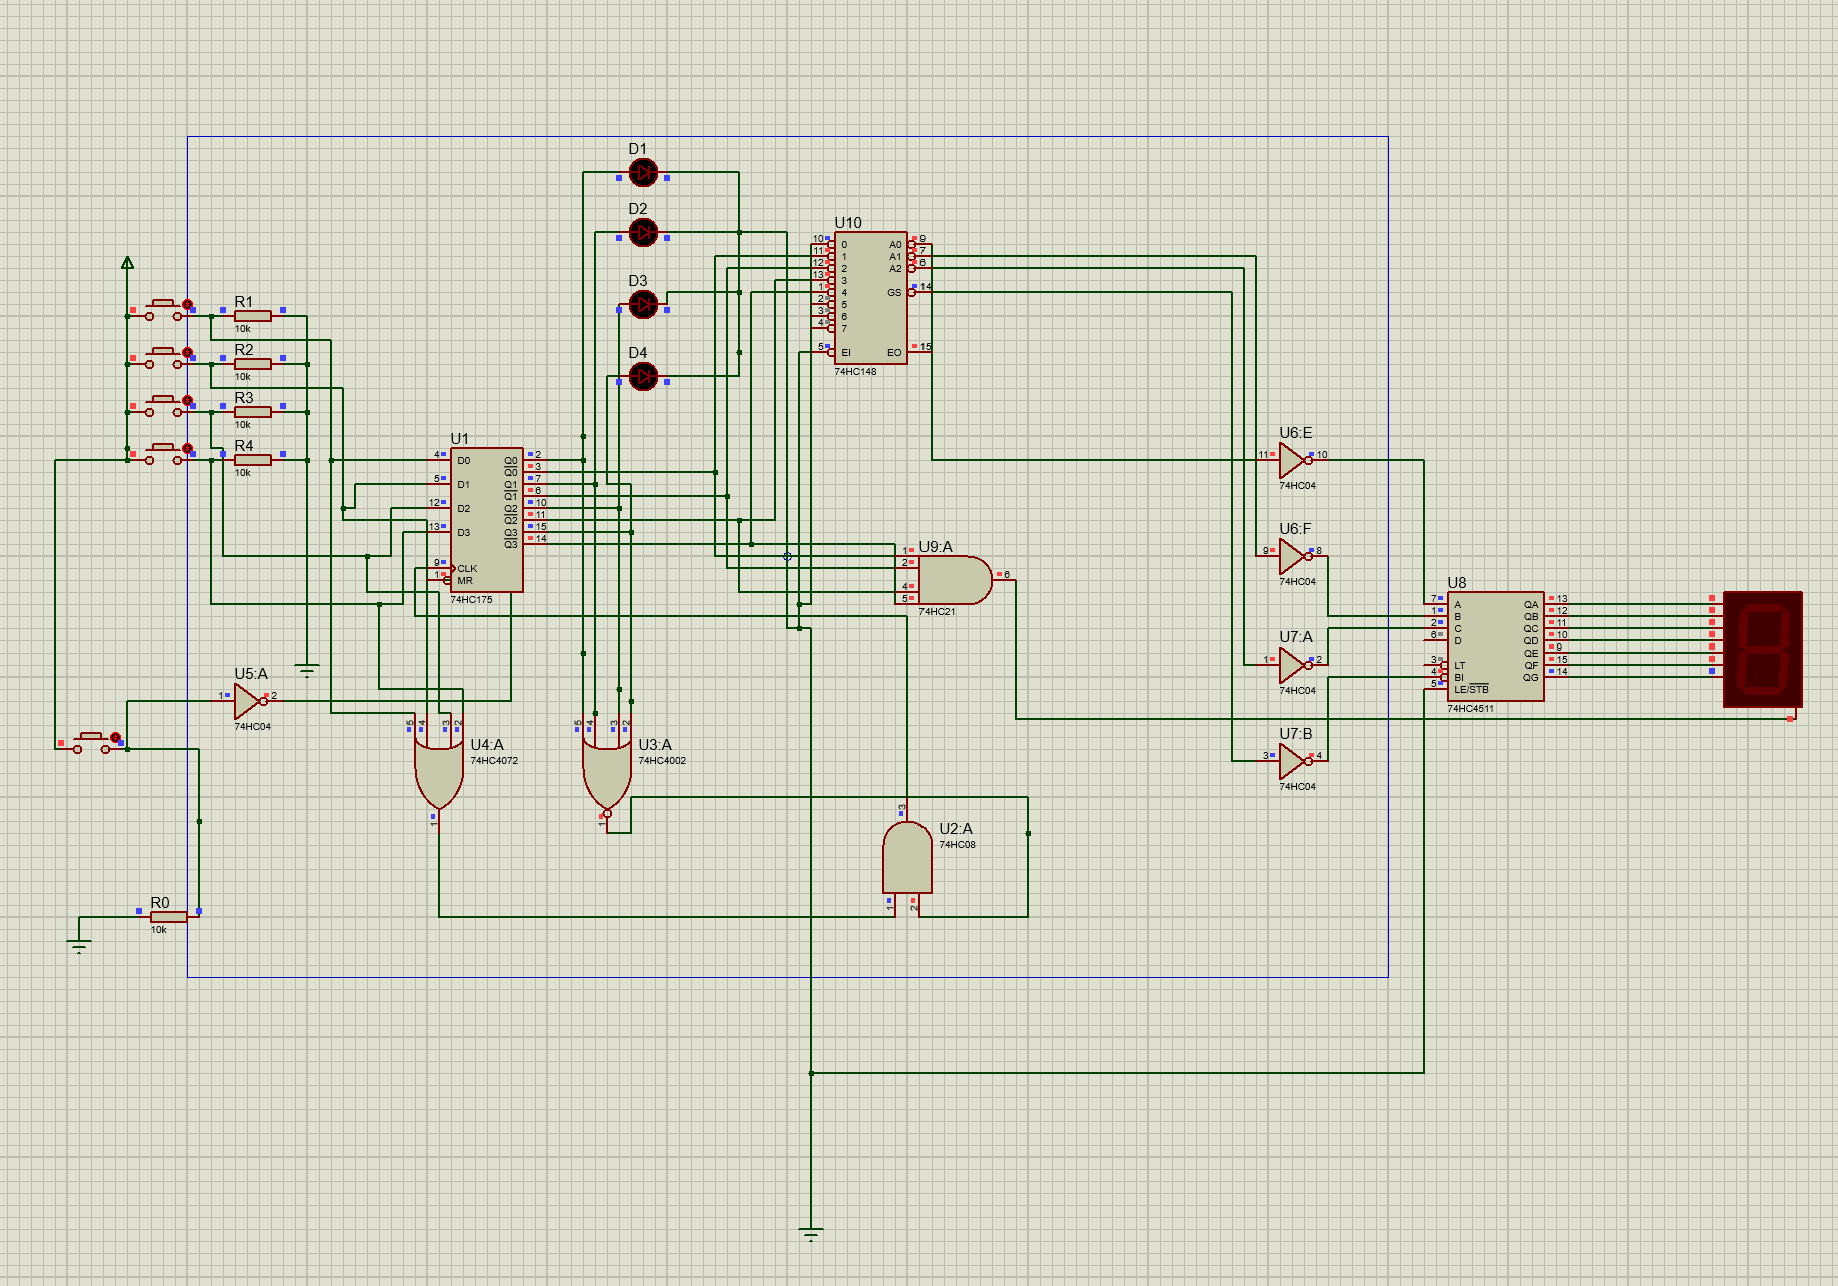
\includegraphics[width=0.75\textwidth]{reset.png} 
    \caption{系统复位清零状态（LED灭，数码管灭）}
\end{figure}

\subsection{1号选手抢答仿真}
复位后，首先闭合1号按键。观察到LED D1点亮，数码管清晰显示数字“1”。保持1号闭合或断开，此时按下2、3、4号按键，电路无任何反应，互锁功能正常
\begin{figure}[H]
    \centering
    % 请将您的1号抢答截图命名为 num1.png 放在同目录下
    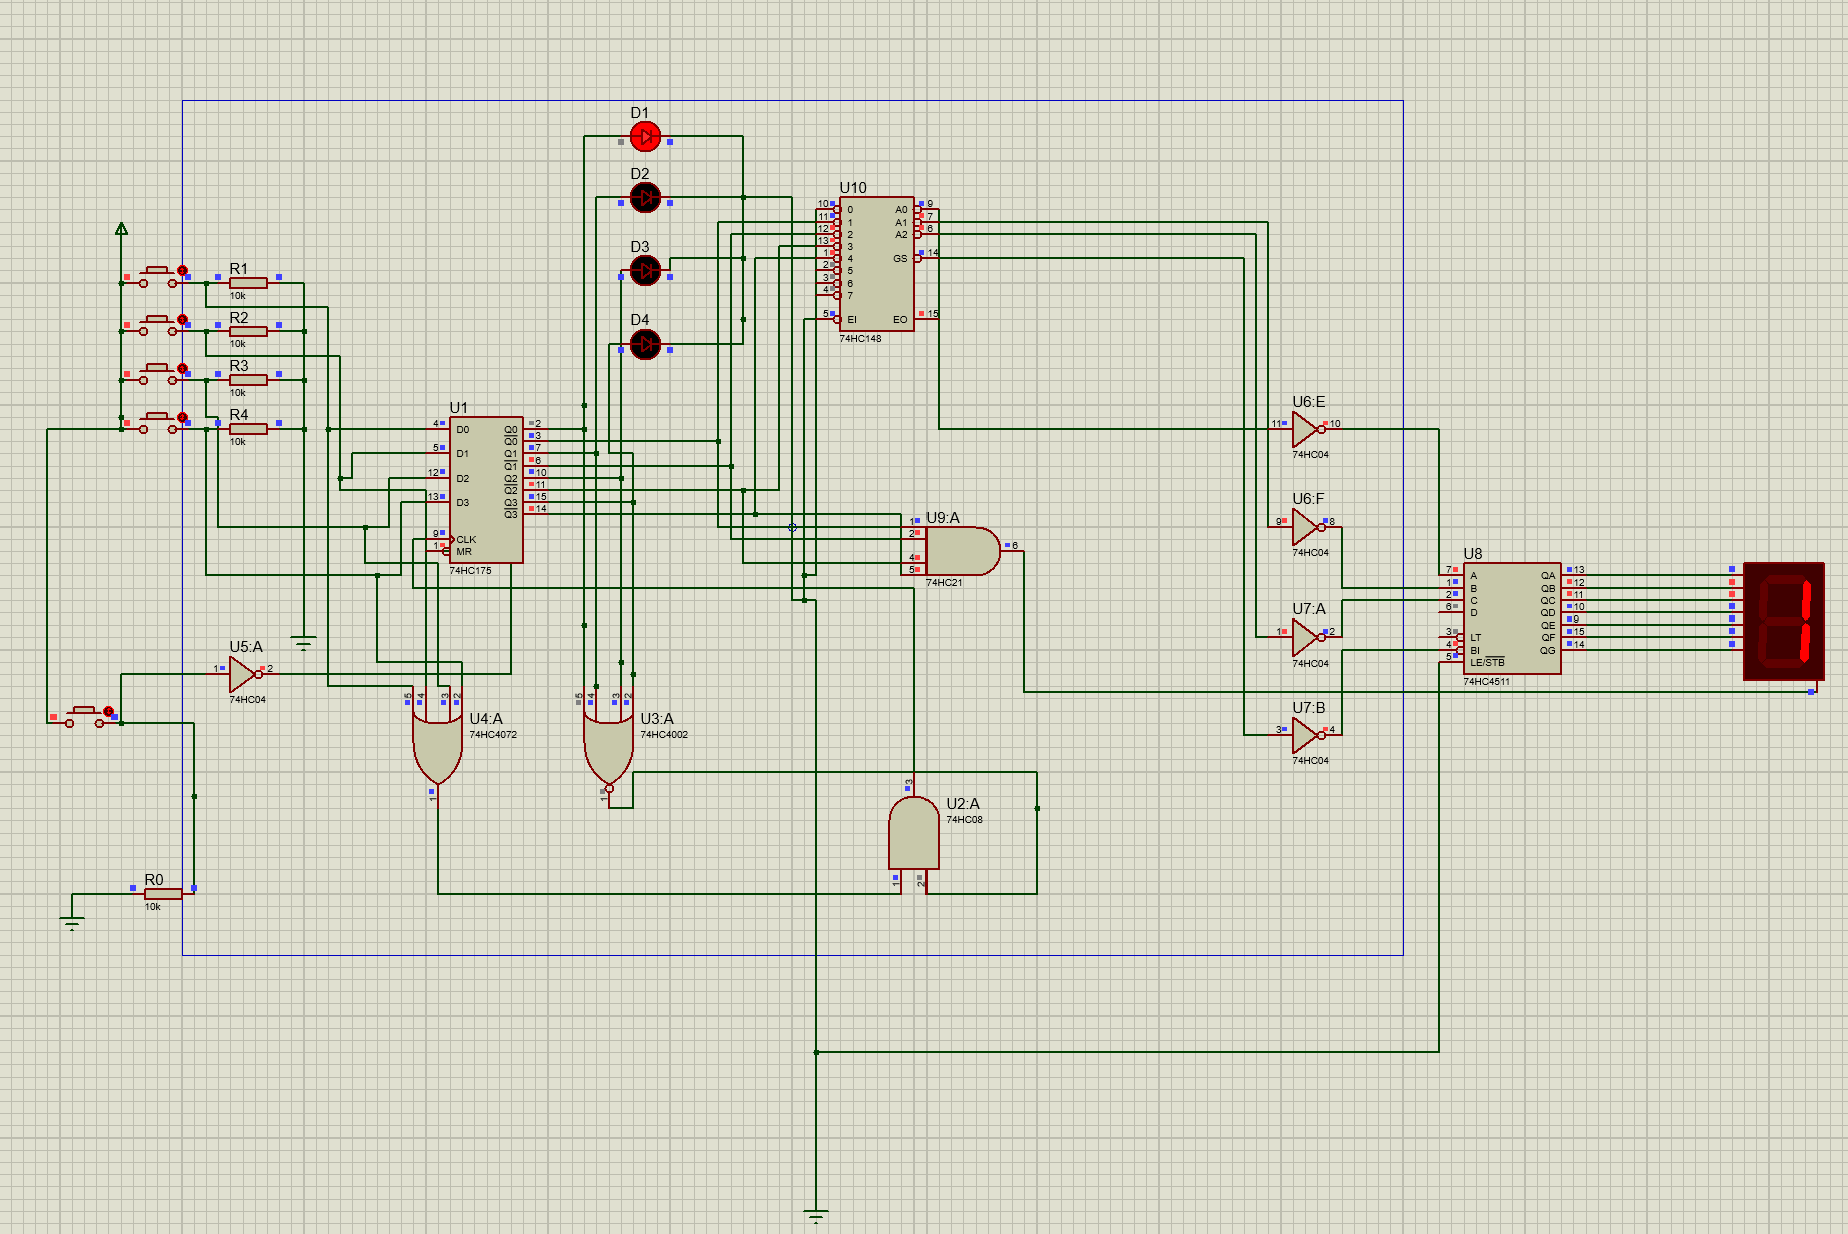
\includegraphics[width=0.75\textwidth]{num1.png} 
    \caption{1号选手抢答成功}
\end{figure}

\subsection{2号及3号选手抢答仿真}
重新按下复位键后，分别单独测试2号和3号按键，均能正确点亮对应LED并显示对应数字，且能成功屏蔽后续其他按键的输入
\begin{figure}[H]
    \centering
    \begin{minipage}[t]{0.48\textwidth}
        \centering
        % 请将您的2号抢答截图命名为 num2.png 放在同目录下
        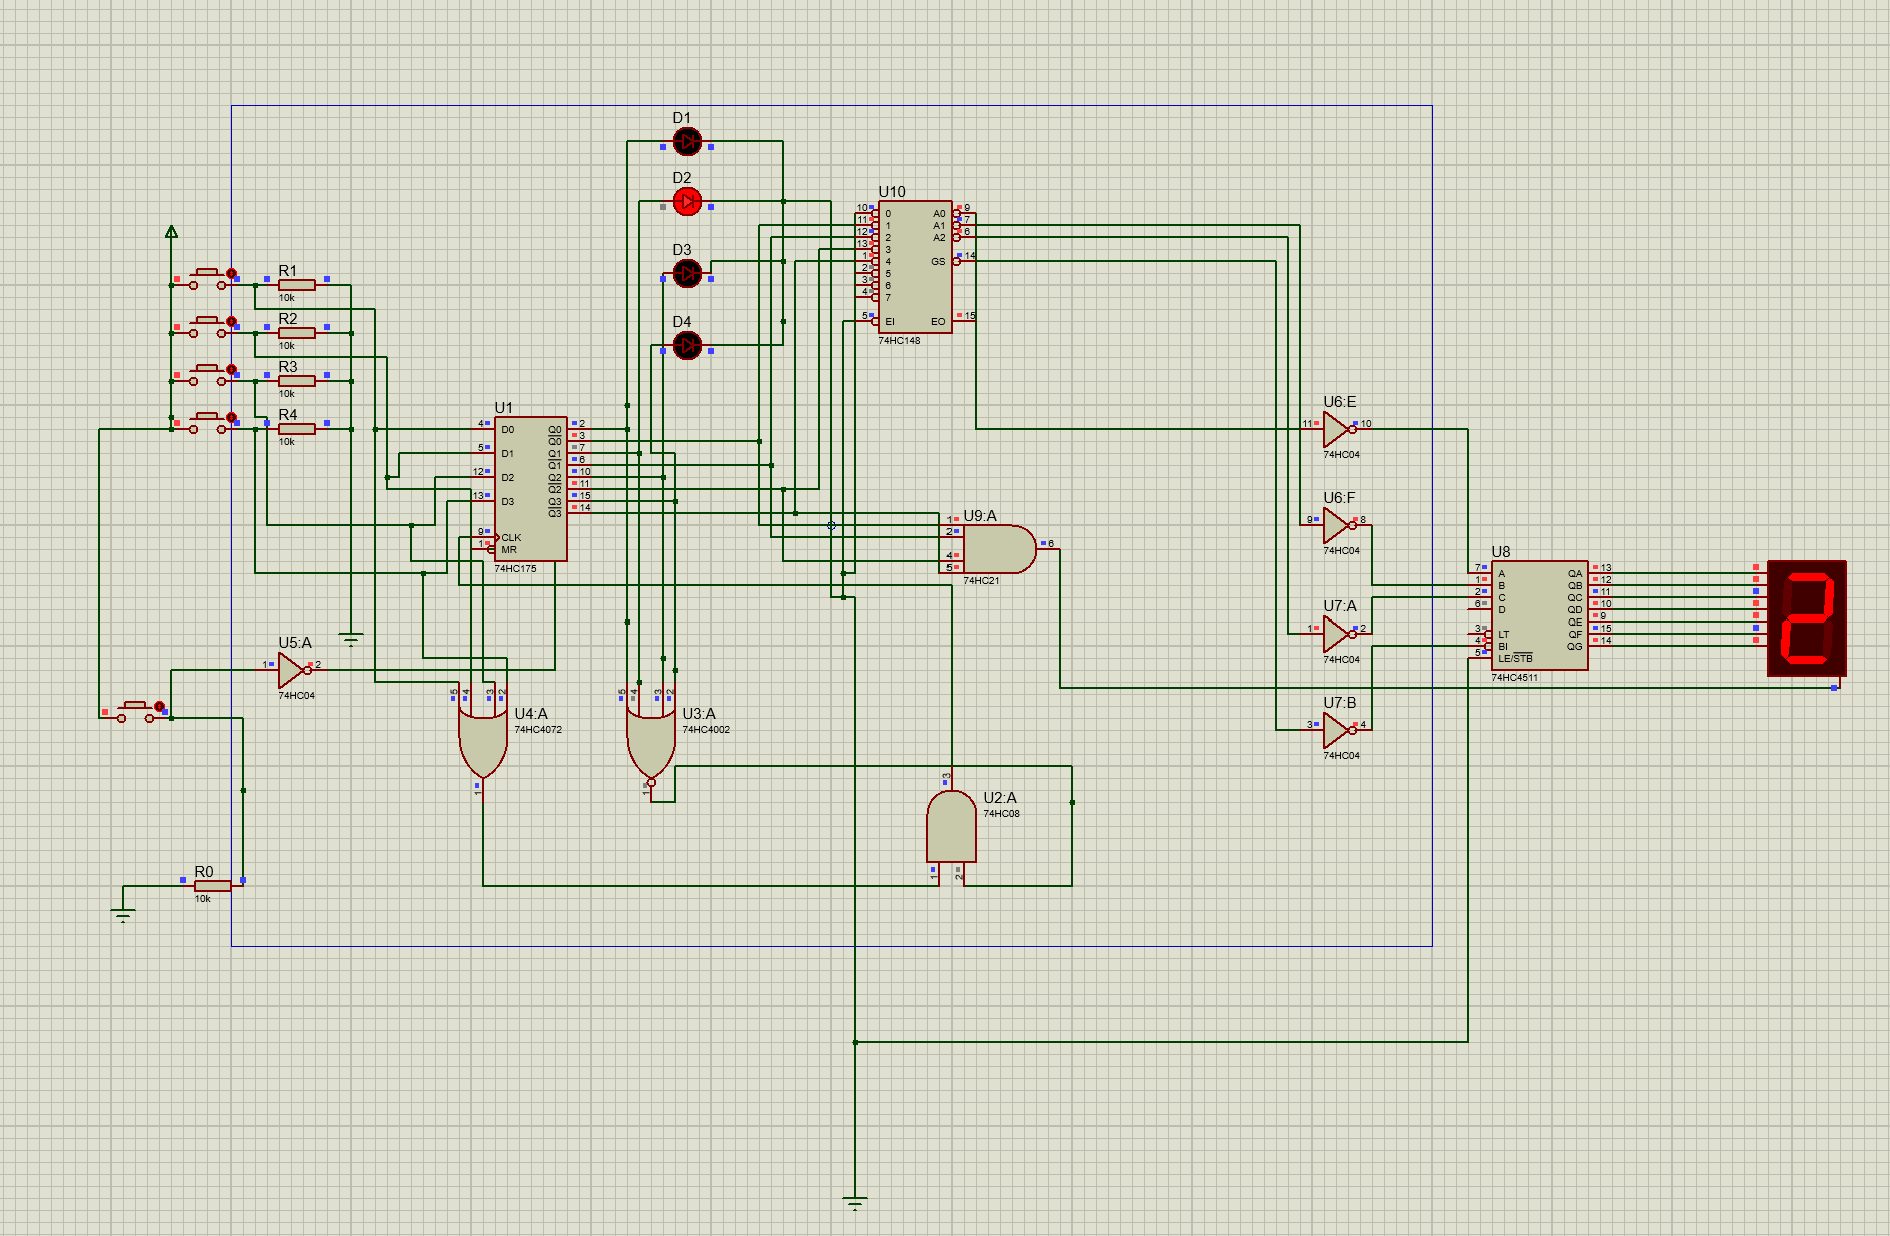
\includegraphics[width=\textwidth]{num2.png}
        \caption{2号选手抢答成功}
    \end{minipage}
    \hfill
    \begin{minipage}[t]{0.48\textwidth}
        \centering
        % 请将您的3号抢答截图命名为 num3.png 放在同目录下
        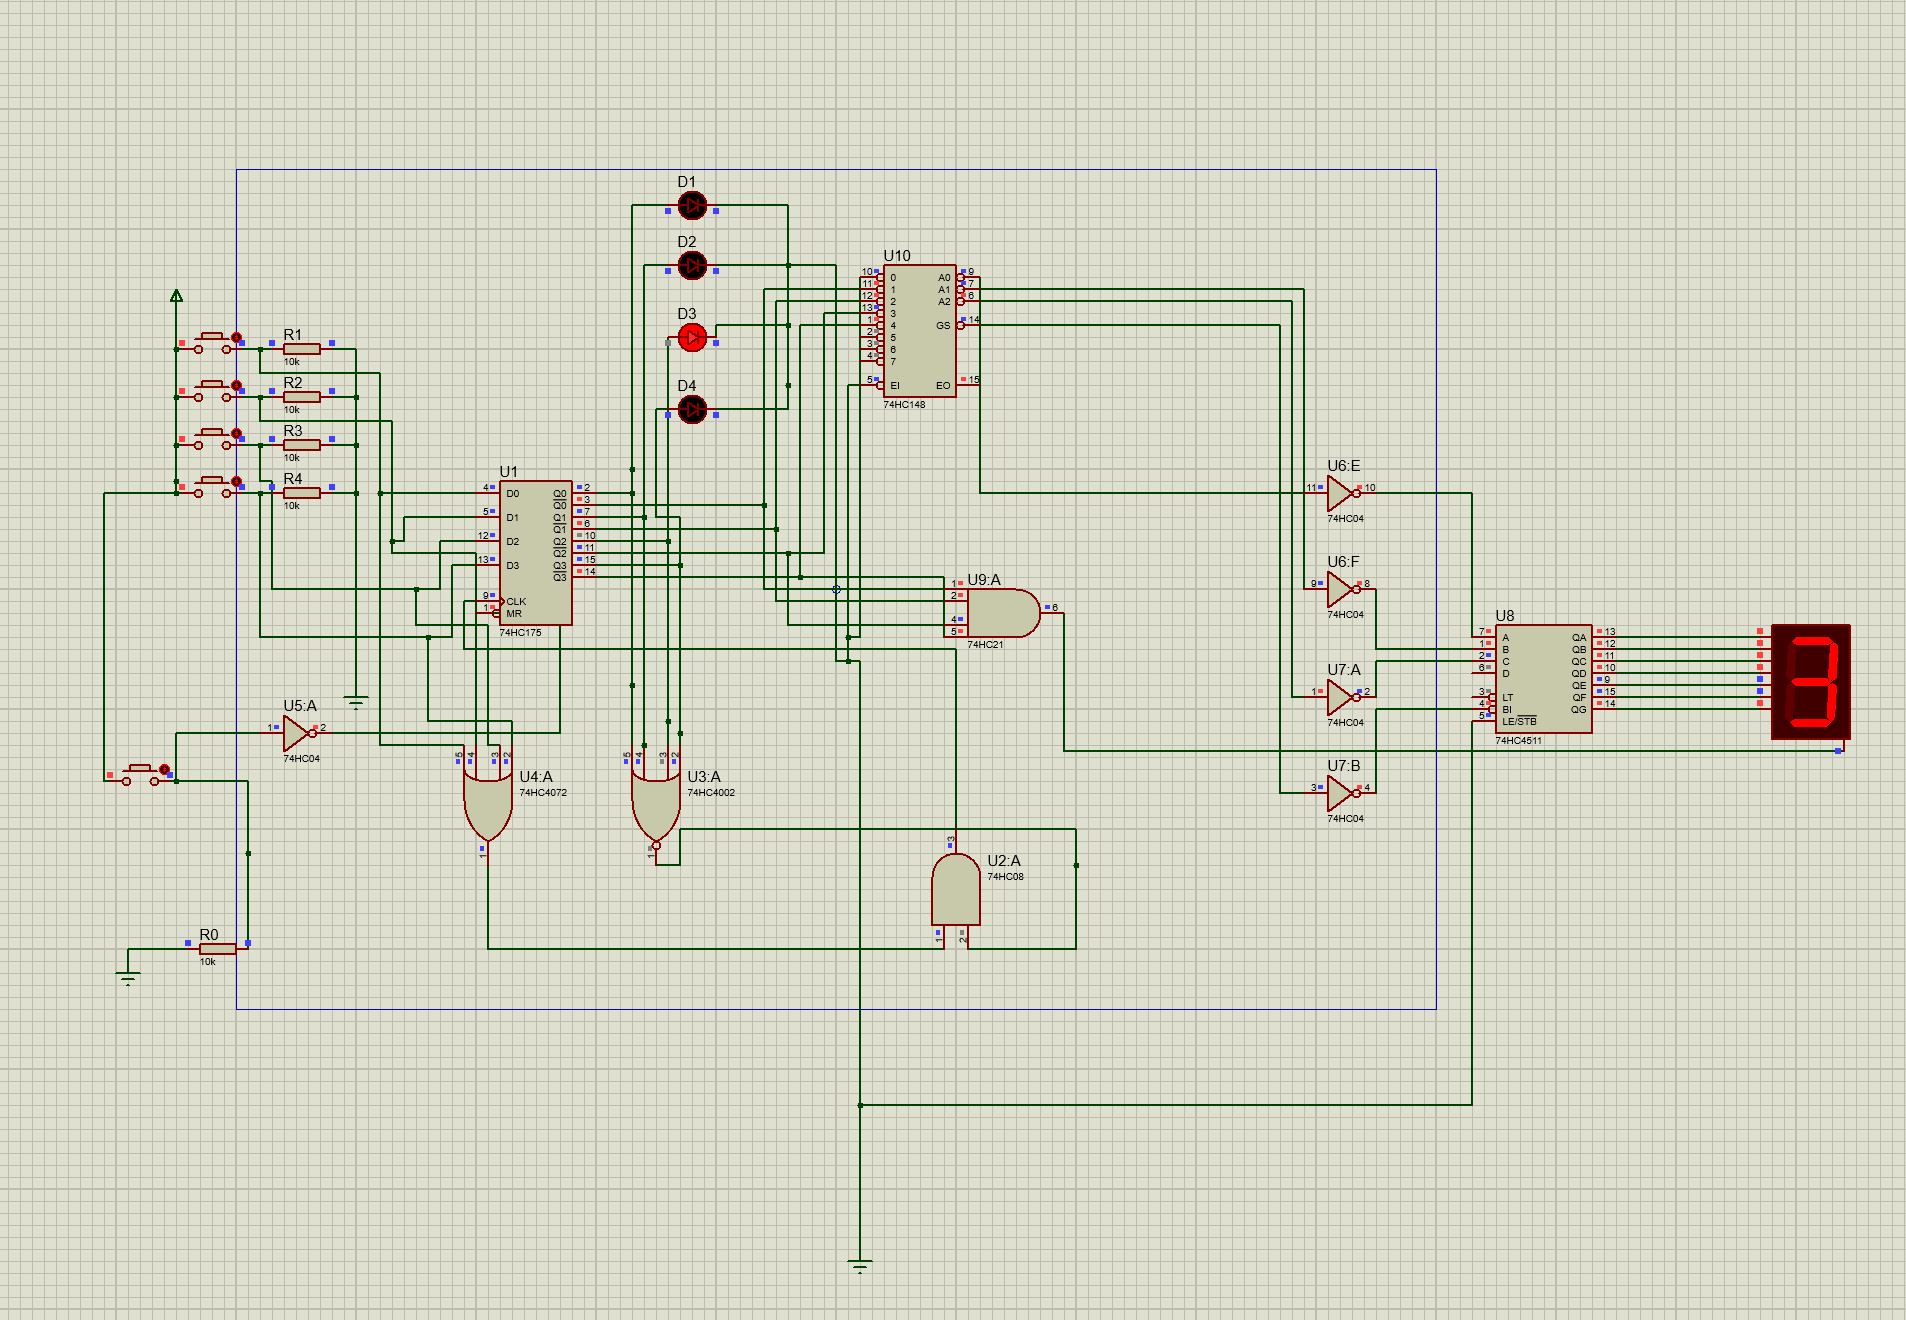
\includegraphics[width=\textwidth]{num3.png}
        \caption{3号选手抢答成功}
    \end{minipage}
\end{figure}

\subsection{4号选手抢答仿真}
按下复位键后，首先按下4号选手按键。如图\ref{fig:num4}所示，D4指示灯点亮，数码管显示数字“4”，充分验证了编码电路引脚连接的正确性
\begin{figure}[H]
    \centering
    % 请将您的4号抢答截图命名为 num4.png 放在同目录下
    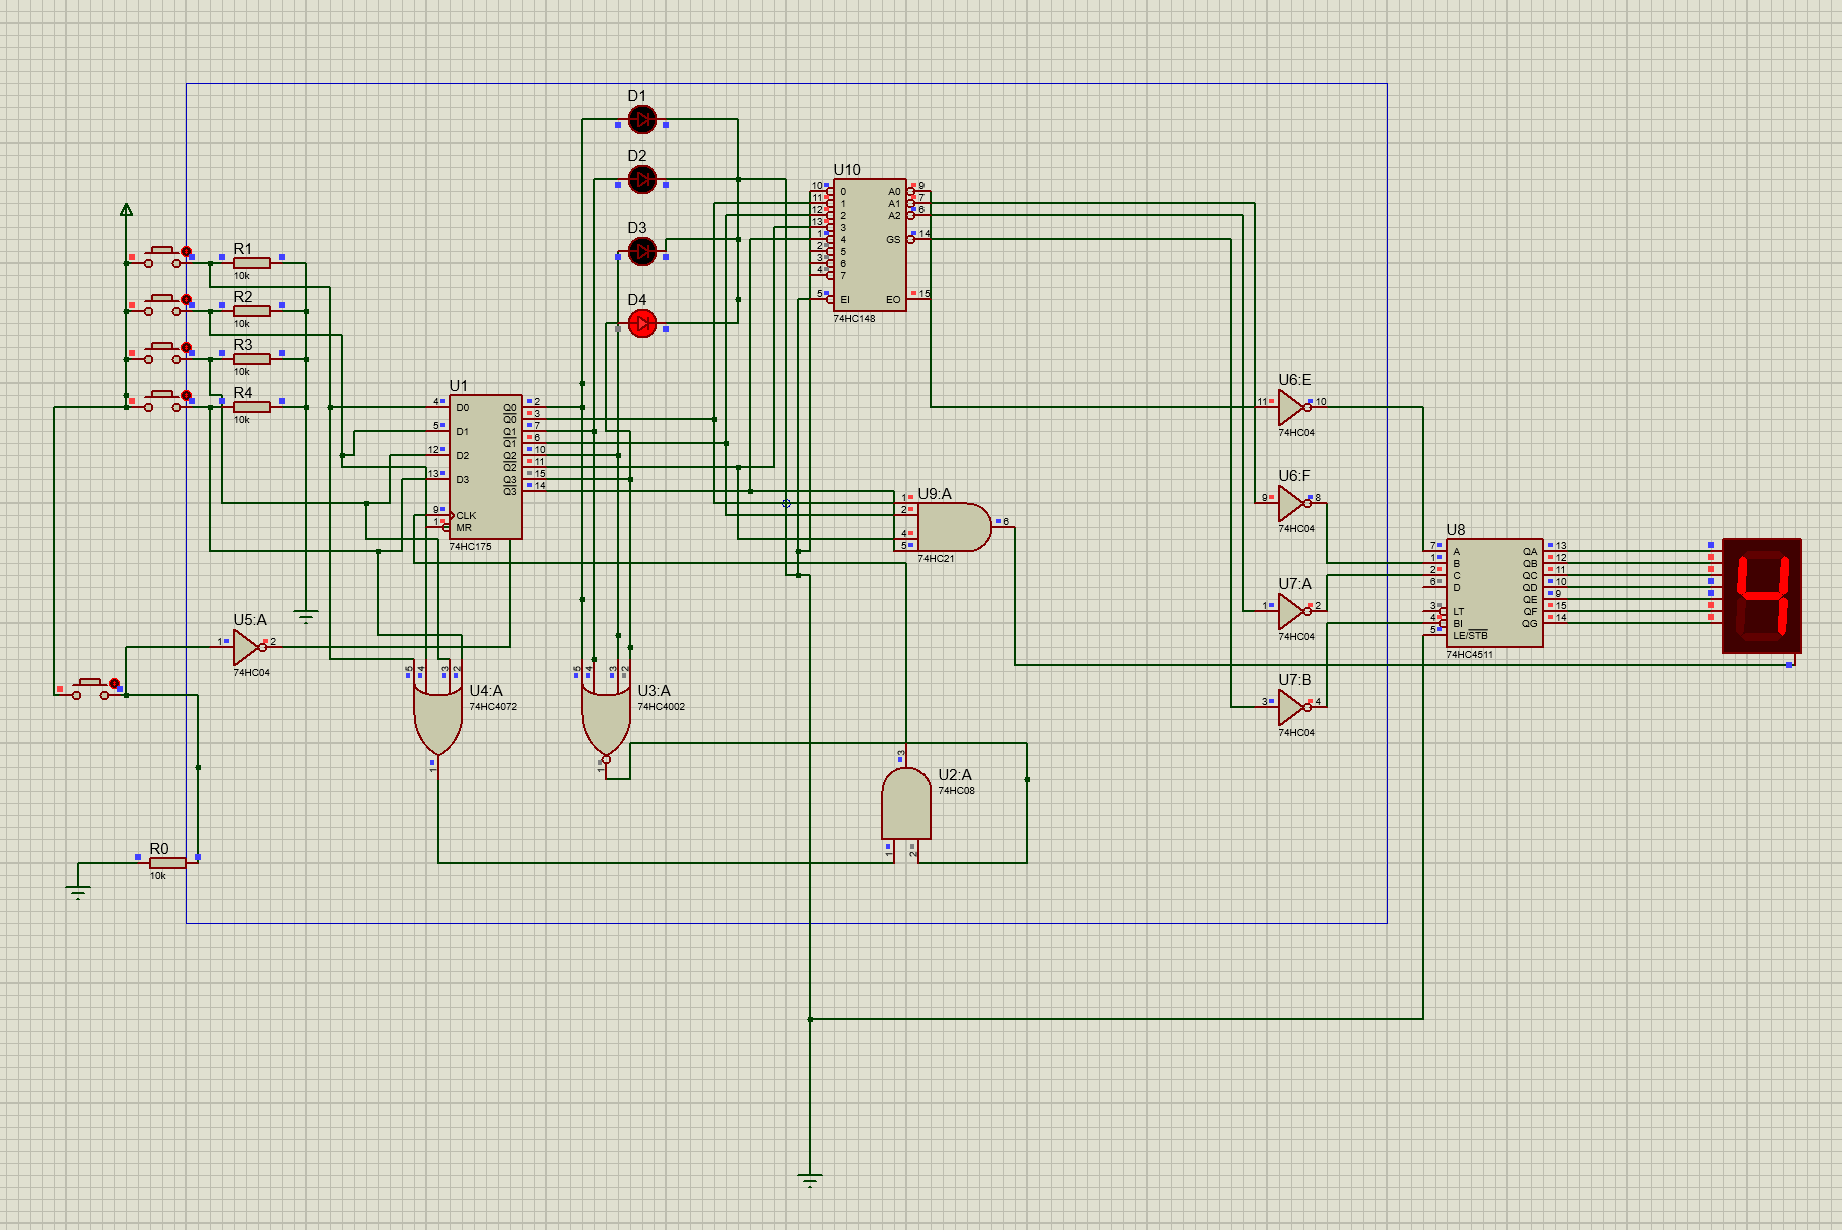
\includegraphics[width=0.75\textwidth]{num4.png} 
    \caption{4号选手抢答成功}
    \label{fig:num4}
\end{figure}


\section{总结}

通过本次开放实验完成了四人抢答器的电路设计与Proteus仿真

\textbf{设计的优势：}
\begin{enumerate}
    \item \textbf{题目要求}：电路没有使用任何单片机等可编程器件，纯靠数字逻辑门（或门、与门、或非门）、触发器、编码器和译码器完成了复杂的逻辑判断
    \item \textbf{细节处理完善}：利用74HC4511的BI引脚实现了复位时的灭灯功能
\end{enumerate}

\textbf{存在的不足与改进方向}
目前的电路仅提供了视觉反馈（LED和数码管）。在实际比赛场景中，通常需要听觉反馈。未来如果条件允许，可以在D触发器的输出端加入一个由555定时器构成的单稳态触发电路，驱动蜂鸣器，使得在抢答成功瞬间能发出短暂的提示音。此外，该电路目前不具备抢答倒计时功能

总体而言，仿真结果与预期设计目标完全一致，验证了电路逻辑的正确性，加深了我对数字电路各种中规模集成芯片（如175、148、4511）组合应用的理解

\end{document}